\section{Task 3: numerical quadrature}
\subsection{Method overview and problem}
Numerical quadrature approximates definite integrals by a weighted sum. The task is to find weights \( Z_i \) and points \( L_i \) satisfying:
\[
\int_a^b f(x)dx \approx \sum_{i=1}^n f(L_i)Z_i,
\]
The points \( L_i \) are evenly spaced over \([a, b]\). The method is derived by requiring the resulting linear system to be exact for polynomials of degree \( n-1 \). For greater precision, \([a, b]\) can be divided into smaller subintervals. These methods form the basis of algorithms for solving problems [sentence unfinished in the original].

\subsection{Solution method}
\begin{enumerate}

\item We want to solve a problem of the form:
\[
    I(f) = \sum_{i = 0}^{n-1} Z_i \cdot f(L(i))  
\]
\item Form the system: construct the appropriate matrix and right-hand-side vector: \[
A_{ij} = L_j^i, \quad B_i = \frac{b^i - a^i}{i}.
\]
\item Solve the linear system \( AZ = B \), described by: \[
\begin{bmatrix}
1 & 1 & \cdots & 1 \\
L_1 & L_2 & \cdots & L_n \\
L_1^2 & L_2^2 & \cdots & L_n^2 \\
\vdots & \vdots & \ddots & \vdots \\
L_1^{n-1} & L_2^{n-1} & \cdots & L_n^{n-1}
\end{bmatrix}
\begin{bmatrix}
Z_1 \\
Z_2 \\
\vdots \\
Z_n
\end{bmatrix} =
\begin{bmatrix}
b-a \\
\frac{b^2-a^2}{2} \\
\frac{b^3-a^3}{3} \\
\vdots \\
\frac{b^n-a^n}{n}
\end{bmatrix}.
\]\noindent 
\item Generate interpolation points: define evenly spaced points as:
\[
L_i = a + i \frac{b-a}{n-1}, \quad i=0,1,\ldots,n-1.
\]
\end{enumerate}
\subsection{Tests} Comparative integration tests covered: \begin{itemize}
    \item Riemann rectangle sums.
    \item Classical quadrature with evenly spaced interpolation points.
    \item Composite quadrature, dividing the interval into smaller parts.
    \item The \texttt{quad} function from \texttt{scipy}.
\end{itemize}
Tests used the interval \([2, 10]\) and functions $\sin(x) + x^2, \ln(x)$:
\begin{enumerate}
    \item Integration error versus interpolation-point count, from 2 to 100.
    \item Points needed to attain a specified precision, with a maximum interpolation count of $25 * (b-a)$.
    \item Convergence of the sum for the interpolated and integrated case, where the integral is known, compared with its approximation.
\end{enumerate}

\begin{minipage}{0.45\textwidth}
    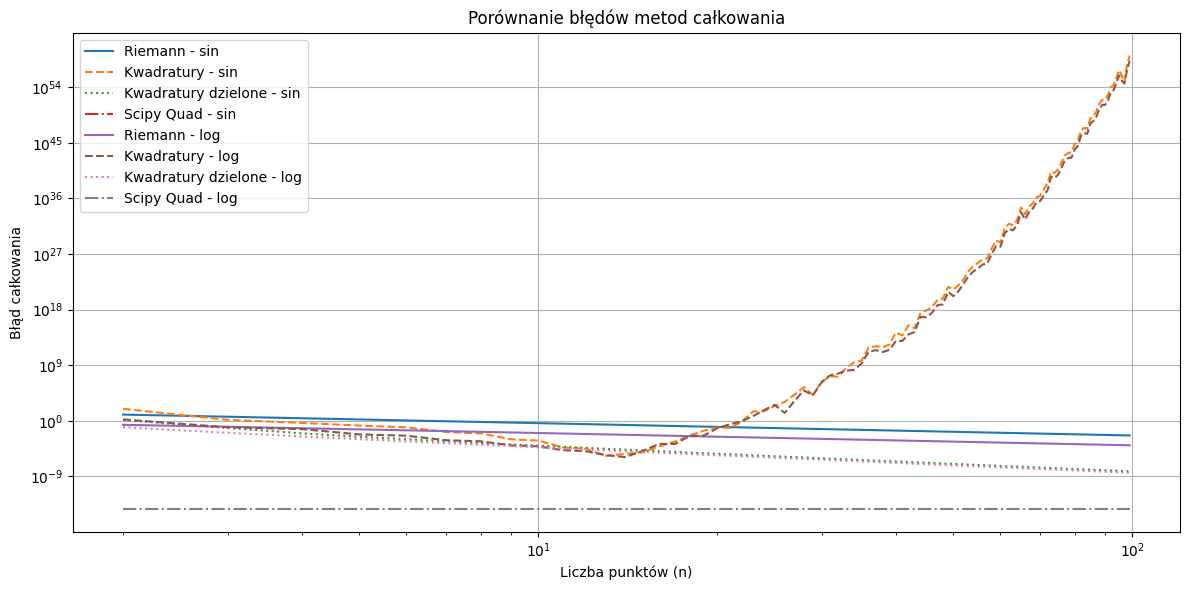
\includegraphics[width=\textwidth]{figures/task-3/error_points-2.png}
\end{minipage} 
\begin{minipage}{0.45\textwidth}
    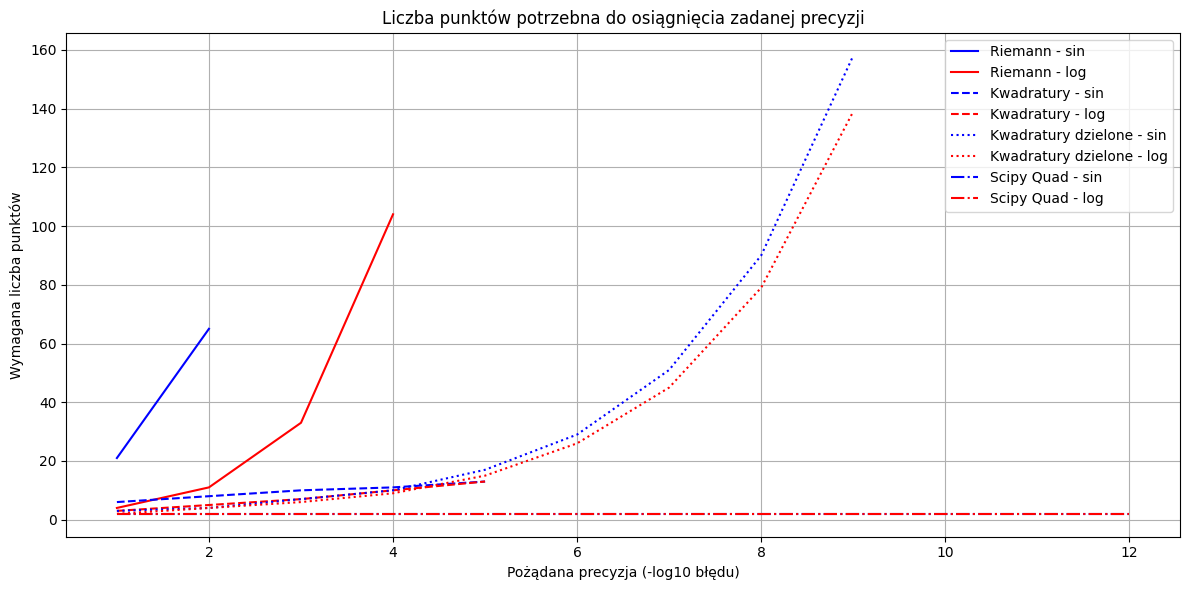
\includegraphics[width=\textwidth]{figures/task-3/points_precision.png}
\end{minipage}

\begin{minipage}{0.92\textwidth}
    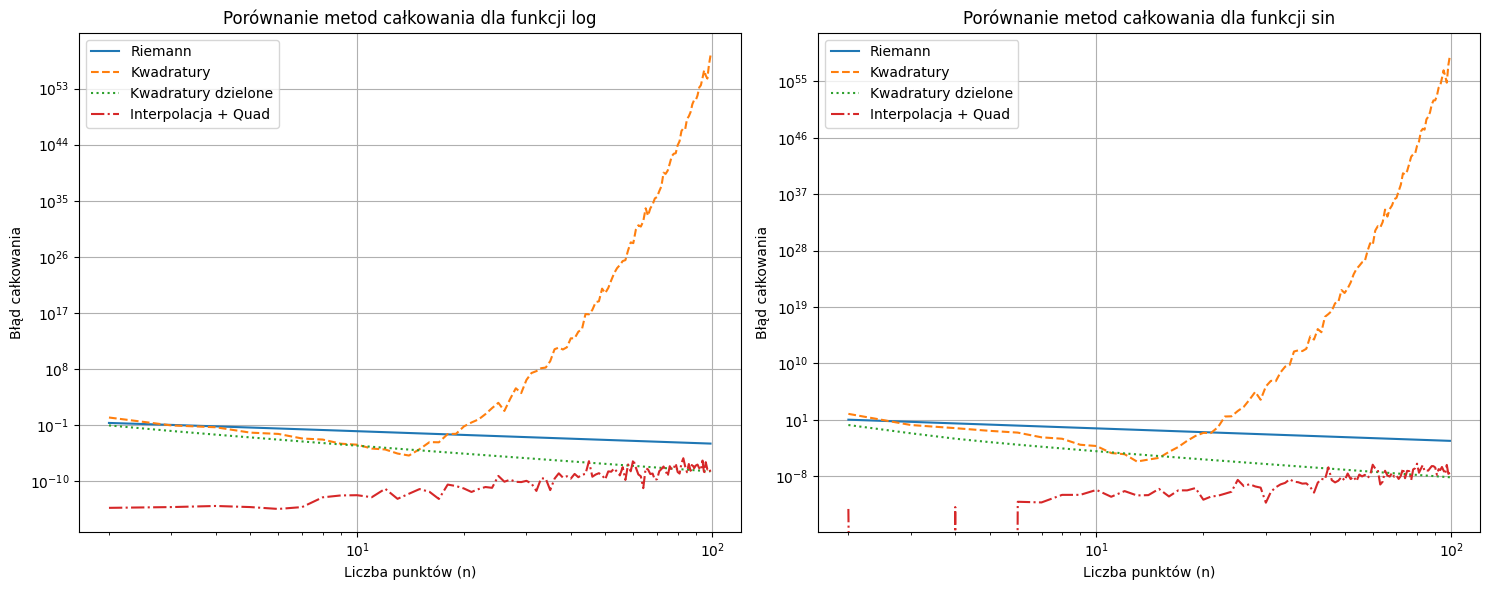
\includegraphics[width=\textwidth]{figures/task-4/error_points.png}
\end{minipage}

\subsection{Conclusions and analysis}
\begin{itemize}
    \item Riemann sums are least efficient and cannot attain the desired precision even with very many points.
    \item Ordinary quadrature is less effective than composite quadrature. It also performs much worse computationally because solving the matrix system is the most expensive operation.
    \item Composite quadrature considerably improves accuracy but is slower and less accurate than the built-in \texttt{quad}.
    \item \texttt{quad} performs best because it selects nonuniform interpolation points and uses Legendre polynomials, enabling accurate approximation of difficult functions.
    \item Computing the interpolating polynomial beforehand is beneficial. The error then depends only on the approximation.
\end{itemize}
\paragraph{Computational complexity}:
\begin{itemize}
    \item Riemann rectangle sums: \( O(n) \).
    \item Classical quadrature: \( O(n^3) \), from solving the linear system.
    \begin{itemize}
        \item Matrix construction: $O(n^2)$.
        \item Linear-system solution: $O(n^3)$, using $LU$.
        \item Therefore the complexity is $O(n^3)$.
    \end{itemize}
    \item Composite quadrature: \( O(k \cdot n^3) \), where \( k \) is the subinterval count and \( n \) is the number of points per subinterval; here \(n=3\).
    \item \texttt{quad}: an adaptive method with nonuniform points. Its complexity depends on the function, but it is efficient in practice because of its use of Legendre polynomials.
\end{itemize}


